\section{Assessing predictive performance}
\label{sec:prediction_model_comparison}

To compare the four prediction methods, we implemented the first two in \pkg{transitr}. The program estimated and saved all arrival time estimates over a full day of data, along with uncertainty and the 5\% and 90\% quantiles. The accuracy of each method is assessed by comparison with the reported arrival times using \gls{rmse}, \gls{mae}, and \gls{mape} (details in \cref{app:error-functions}). Since predictions change over time, we also computed the summary values by \emph{time until (actual) arrival}, allowing the comparison of models at different time points, as well as by stop sequence and time of day.


Another useful criteria is the \gls{picp}, which is only available for the three methods that provide an 85\% \gls{ppi}: for the particle filter, this is achieved by sorting the particles in order of arrival time and taking the $\lfloor 0.05 N^\star\rfloor^{\text{th}}$ particle as the lower bound, and the $\lceil 0.9 N^\star\rceil^{\text{th}}$ particle as the upper bound (more details in \cref{app:particle-summaries}). For the Normal approximation and historical arrival methods, the inverse \gls{cdf} provides the required quantiles. The results are displayed in \cref{tab:model_results_rmse} and \cref{fig:model_results_rmse_time,fig:model_results_rmse_stopn,fig:model_results_rmse_timeofday} and described in \cref{sec:prediction_model_comp_stats}.


Additionally, we want to compare the reliability of the various forecast methods, namely \emph{the probability of arriving before the bus}, and hence not missing it, as well as the expected waiting time given a passenger arrives at the stop by a certain time. \Cref{tab:model_results_pr_miss} and \cref{fig:model_results_pr_gtfs,fig:model_results_pr_time,fig:model_results_pr_stop,fig:model_results_pr_timeofday} use the point estimate (mean or median, depending on the forecast method) and the 5\% quantile to calculate the probability that the bus arrives after each estimate. \Cref{sec:prediction_model_comp_probs} discusses these results.





\begin{knitrout}\small
\definecolor{shadecolor}{rgb}{0.969, 0.969, 0.969}\color{fgcolor}\begin{table}

\caption[Comparison of the predictive performance of the four methods after estimating arrival times for a full day of historical data]{\label{tab:model_results_rmse}Comparison of the predictive performance of the four methods after estimating arrival times for a full day of historical data. RMSE, MAE, and MAPE measure the accuracy of the mean or median, and PICP measures the accuracy of the distribution: the nominal coverage is 85\% (PICP is not available for the schedule-delay method).}
\centering
\fontsize{8}{10}\selectfont
\begin{tabular}[t]{lrrrr}
\toprule
  & RMSE (s) & MAE (s) & MAPE (\%) & PICP (\%)\\
\midrule
\Fpf{}: Particle filter & 232 & 146 & 19 & 77\\
\Fnorm{}: Normal approximation & 489 & 349 & 38 & 91\\
\Fhist{}: Historical delays & 244 & 166 & 47 & 84\\
\Fsched{}: Schedule-delay & 238 & 164 & 27 & \\
\bottomrule
\end{tabular}
\end{table}


\end{knitrout}




\subsection{Comparing the accuracy of arrival time prediction}
\label{sec:prediction_model_comp_stats}

The accuracy measurements (\gls{rmse}, \gls{mae}, and \gls{mape}) shown in \cref{tab:model_results_rmse} immediately show that the Normal approximation (\Fnorm{}) estimates are, on average, about half as accurate as the other methods. Overall, the \pf{} (\Fpf{}) demonstrates the greatest accuracy by all criteria, indicating that its estimates are (on average) closer to the true value in both absolute and relative terms. The historical delays approach (\Fhist{}) has similar accuracy to the schedule-delay approach (\Fsched{}) in absolute terms (\gls{rmse} and \gls{mae}), but the least accurate overall in relative terms (\gls{mape}). This indicates that \Fhist{} has worse accuracy for short-term forecasts, which is not surprising as it uses only historical data, ignoring \rt{} information about vehicle location and network state.


As for the \gls{picp}, the theoretical coverage is 85\%. \Fpf{} underestimates arrival time uncertainty, indicating that the model is not capturing enough uncertainty: this could be any combination of dwell time, travel time, or the unknown. Conversely, \Fnorm{} overestimates uncertainty by about 5\%. \Fhist{} has close to the desired \gls{picp}, which demonstrates that arrival time delays at each stop show a certain level of consistency from day-to-day.


The main finding of \cref{tab:model_results_rmse} is that the Normal approximation is inadequate for this problem. However, this was not unexpected: in previous chapters, I emphasised the non-Gaussian nature of a vehicle's state. We now explore the effects of time-until-arrival, stop sequence, and time-of-day on prediction accuracy to more closely inspect the relative performance of the methods.


\subsubsection{Time until actual arrival}

We would expect arrival time predictions for a given stop to become more accurate as the bus approaches. To assess this, arrival time estimates were binned into one-minute intervals, and for each, the summary statistics were estimated, which are displayed in \cref{fig:model_results_rmse_time}. Note the use of log scales for \gls{rmse}, \gls{mae}, and \gls{mape}.


\begin{knitrout}\small
\definecolor{shadecolor}{rgb}{0.969, 0.969, 0.969}\color{fgcolor}\begin{figure}
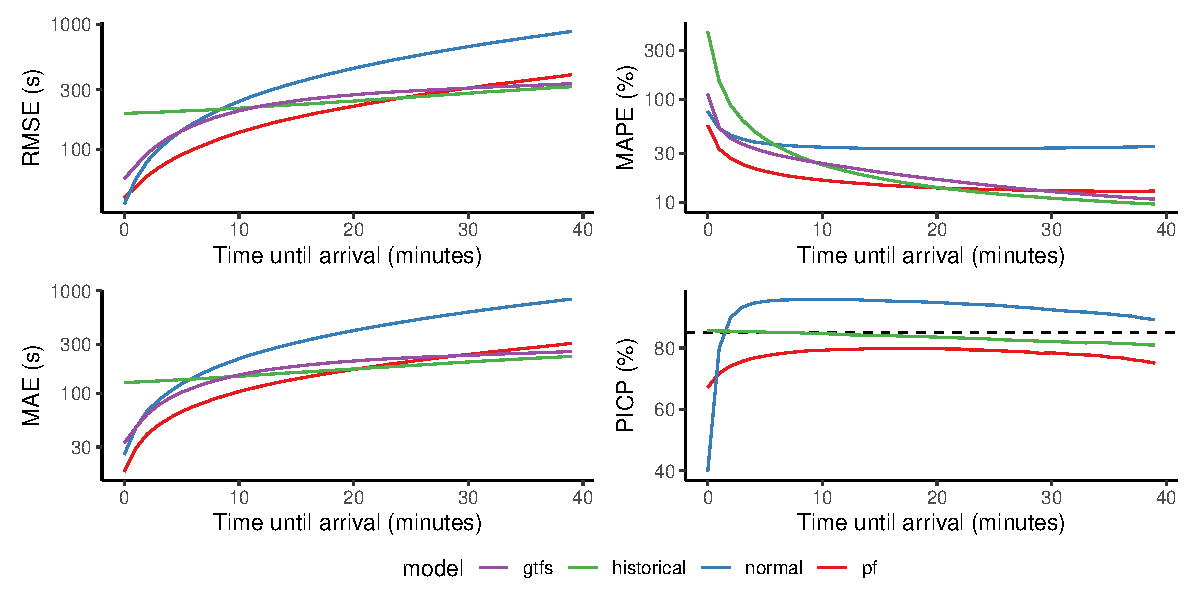
\includegraphics[width=\textwidth]{figure/model_results_rmse_time-1} \caption[Model comparative statistics as a function of time until arrival]{Model comparative statistics as a function of time until arrival. Note the log-scale for RMSE, MAE, and MAPE. The dashed line in the graph of PICP indicates the nominal coverage of 85\%.}\label{fig:model_results_rmse_time}
\end{figure}


\end{knitrout}

The \gls{rmse} and \gls{mae} for all methods increase with time until arrival as expected. The rate of this increase, however, varies between them. The three methods that use \rt{} information (\Fpf{}, \Fnorm{}, and \Fsched{}) demonstrate small absolute error when the bus is near, which increases the farther out the bus gets, while \Fhist{} shows a more constant error and far poorer accuracy when the bus is less than 5--10~minutes away. \Fpf{} has the lowest error up until 20~minutes before arrival and has greater accuracy than \Fsched{} up until 25--30~minutes. This indicates that the current delay is only a useful predictor when the bus has almost arrived, and that accounting for \rt{} traffic conditions does improve the accuracy of arrival time prediction. \Fnorm{} quickly shows large prediction errors for all but the nearest buses.



The \gls{mape} for all methods decreases with time until arrival, with \Fhist{} showing the highest relative error when the bus is less than about 5~minutes away. \Fnorm{} remains somewhat constant with a relative error of about 50\%. Again, for the first 20~minutes, \Fpf{} has the smallest relative error, and outperforms \Fsched{} up until the bus is 25--30~minutes away. After 30~minutes, \Fpf{} converges with slightly lower accuracy than \Fhist{} and \Fsched{}, which may continue to decrease beyond 40~minutes. However, 89\% of routes in Auckland are less than one hour, so the number of arrival time predictions made when the bus is more than 40~minutes away is small so results will be strongly affected by individual routes.


The \gls{picp} is not available for \Fsched{} since that method only provides point estimates. The coverage for the three remaining methods is reasonably constant across time until arrival (\cref{fig:model_results_rmse_time}). As seen earlier, \Fpf{} underestimates arrival time uncertainty, noted by lower than expected coverage. \Fnorm{} overestimates uncertainty when the bus is more than a few minutes away, and thoroughly underestimates uncertainty when the bus is near, likely because it does not account for enough vehicle state uncertainty. \Fhist{} exhibits good coverage, although this drops slightly as time-until-arrival increases.


\subsubsection{Stop sequence}

\Cref{fig:model_results_rmse_stopn} shows the \gls{rmse}, \gls{mae}, \gls{mape}, and \gls{picp} grouped by stop sequence. The first stop is excluded since arrival times are only predicted once the bus begins the trip. Early stops along a route seldom have long until the bus arrives since \glspl{eta} are only made once the trip starts. Stop sequence is truncated to 50 (92\% of trips have fewer than that many stops).


\begin{knitrout}\small
\definecolor{shadecolor}{rgb}{0.969, 0.969, 0.969}\color{fgcolor}\begin{figure}
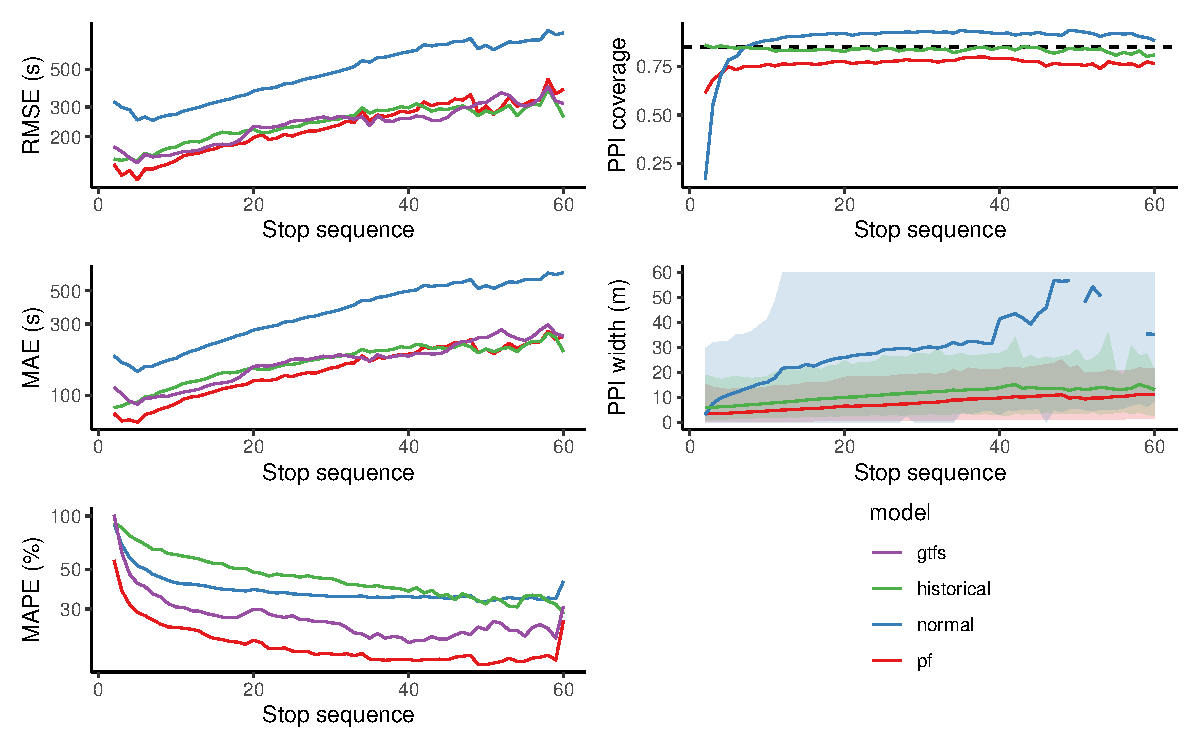
\includegraphics[width=\textwidth]{figure/model_results_rmse_stopn-1} \caption[Model comparative statistics as a function of stop sequence]{Model comparative statistics as a function of stop sequence. RMSE, MAE, and MAPE once more use a log-scale. The dashed line in the graph of PICP indicates 85\% nominal coverage.}\label{fig:model_results_rmse_stopn}
\end{figure}


\end{knitrout}

Both \gls{rmse} and \gls{mae} increase with stop sequence for all models. \Fnorm{} shows much higher errors than the other three methods, and \Fpf{} exhibits higher prediction accuracy than \Fhist{} and \Fsched{} up until about stop 30, at which point there is no clear difference between these three methods. However, in terms of relative error (\gls{mape}), \Fpf{} outperforms the others for all stops, while \Fhist{} shows the poorest accuracy, particularly for early stops.


\Gls{picp} shows much the same trend as before with \Fpf{} underestimating arrival time uncertainty at all stops, while \Fnorm{} overestimates for all but the first few stops---it performs poorly for those. \Fhist{} has the desired coverage for all stops.


\subsubsection{Time of day}

Observations were binned into 15-minute intervals and summary statistics calculated for each. The results, displayed in \cref{fig:model_results_rmse_timeofday}, differ from those seen previously, now revealing the peak-hour traffic effect. There is a single morning peak at around 8~am (school and work begin at about the same time) and two evening peaks: one for schools at about 3~pm, and another for workers at around 5~pm.


\begin{knitrout}\small
\definecolor{shadecolor}{rgb}{0.969, 0.969, 0.969}\color{fgcolor}\begin{figure}
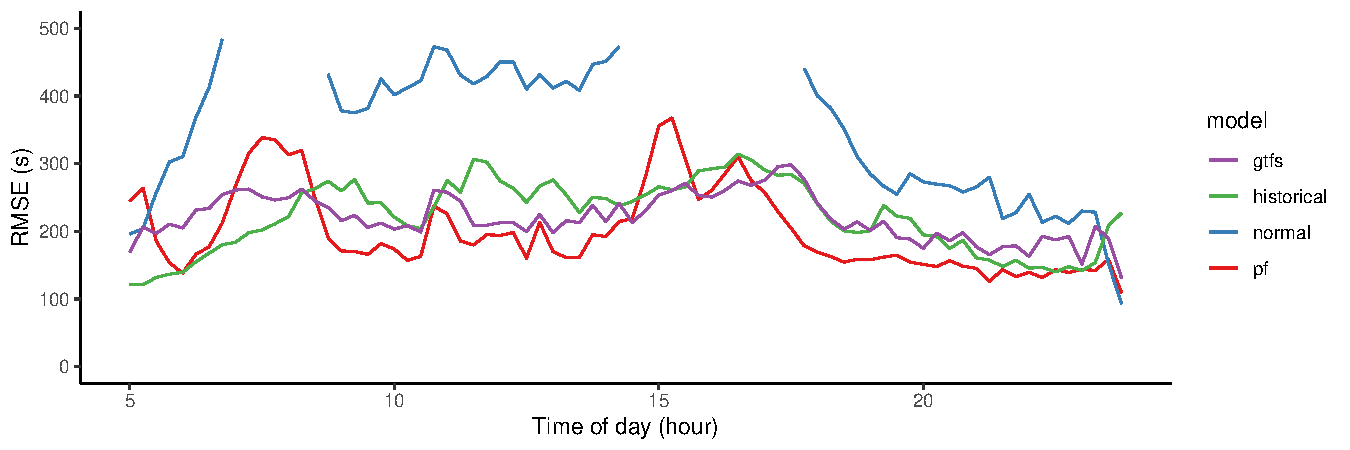
\includegraphics[width=\textwidth]{figure/model_results_rmse_timeofday-1} \caption[Model comparative statistics as a function of time of day]{Model comparative statistics as a function of time of day. RMSE, MAE, and MAPE use log-scales, and the dashed line in the graph of PICP indicates 85\% nominal coverage.}\label{fig:model_results_rmse_timeofday}
\end{figure}


\end{knitrout}

During off-peak (about 9:30~am until 2:30~pm) \Fpf{} shows the smallest error (\gls{rmse} and \gls{mae}), with \Fhist{} and \Fsched{} exhibiting slightly larger errors. \Fnorm{} again has much poorer accuracy\footnote{Remember to note the log scale.}. During peak times, all methods show an increase in prediction error as traffic conditions worsen and become more unreliable. \Fsched{} is least affected by the peak effect since the schedules do account somewhat for peak congestion, while the current implementation of our method only uses the \emph{current} traffic state; however, as discussed in \cref{sec:nw_hist_model}, improvements could be achieved by implementing a better forecast method.

In terms of relative error (\gls{mape}), we see a less accentuated peak effect, and now \Fpf{} demonstrates the best accuracy throughout the day. During peak time, traffic can quickly become more or less congested, so long-term predictions are prone to inaccuracy as we saw in \cref{fig:model_results_rmse_time}. Therefore, peak traffic has a noticeable effect on \gls{rmse} and \gls{mae}, but less so on \gls{mape}. \Gls{mape} for \Fsched{} and \Fhist{} seems unaffected by peak hour.


Finally, we look to \gls{picp}, where we can truly see the effect of peak traffic on the predicted arrival time distributions, particularly when obtained using \Fpf{}. During off-peak, \Fpf{} has very close to the desired coverage of 85\%; during peak time, however, coverage drops quite significantly. This drop is likely caused by travel times quickly increasing as congestion builds, meaning initial predictions are too early, and then as travel times decrease again once peak time has passed, the predictions are too late. Our \pf{} appears to be able to estimate travel times accurately, but it would benefit from the forecasting improvement described in \cref{sec:nw_hist_model}.\footnote{Which we were, unfortunately, unable to complete at this time.}




\subsection{Assessing the reliability of arrival time prediction}
\label{sec:prediction_model_comp_probs}

\Gls{rmse}, \gls{mae}, and \gls{mape} measure the predictive accuracy of the methods, but do not account for the costs associated with inaccurate predictions. In this section, we evaluate the \emph{reliability} of arrival time distributions by examining:
\begin{enumerate}
\item the wait time at the bus stop; and
\item the probability of missing the target bus.
\end{enumerate}
In most cases, the latter incurs a much higher cost, but depends entirely on time until the \emph{next} bus arrival: for high-frequency routes, this is small; for low-frequency ones, however, it can become quite high.\footnote{Some routes only run hourly!} In this section, I do not differentiate between high and low-frequency routes (I do in \cref{sec:eta_estimates}, however).


The three statistics we compare across the methods are:
\begin{itemize}
\item $\mathbb{P}_m = \Pr{\Varr_m \geq \hat\Tarr_m}$, the probability that the vehicle arrives after the point estimate, $\hat\Tarr_m$, indicating that were a passenger to arrive at the stop by $\hat\Tarr_m$, they would catch the bus with probability $\mathbb{P}_m$;
\item $\mathbb{P}_\ell = \Pr{\Varr_m \geq \hat\alpha_{m,\text{lower}}}$, the probability that the vehicles arrives after the lower bound of the \gls{ppi}; and
\item $\mathbb{E}_\ell = \E{\Varr_m - \hat\alpha_{m,\text{lower}} | \Varr_m \geq \hat\alpha_{m,\text{lower}}}$, the expected waiting time for a passenger arriving at the lower predictive bound, given that the bus arrives after it (that is, conditional on catching the bus).
\end{itemize}


\begin{knitrout}\small
\definecolor{shadecolor}{rgb}{0.969, 0.969, 0.969}\color{fgcolor}\begin{table}

\caption[Comparison of the reliability of the four prediction methods based on the results of estimating arrival times for a full day of historical data]{\label{tab:model_results_pr_miss}Comparison of the reliability of the four prediction methods based on the results of estimating arrival times for a full day of historical data. $\mathbb{P}_m$ and $\mathbb{P}_\ell$ are proportions of observed events, and $\mathbb{E}_\ell$ and its associated interval are based on the mean and quantiles.}
\centering
\fontsize{8}{10}\selectfont
\begin{tabular}[t]{lrrrl}
\toprule
  & $\mathbb{P}_m$ (\%) & $\mathbb{P}_\ell$ (\%) & $\mathbb{E}_\ell$ (m) & 5--90\% CI\\
\midrule
\Fpf{}: Particle filter & 64 & 93 & 4.4 & 0.3--10.2\\
\Fnorm{}: Normal approximation & 96 & 98 & 20.9 & 2.9--37.6\\
\Fhist{}: Historical delays & 54 & 98 & 7.1 & 1.1--14.1\\
\Fsched{}: Schedule-delay & 38 &  &  & \\
\bottomrule
\end{tabular}
\end{table}


\end{knitrout}

The overall results are displayed in \cref{tab:model_results_pr_miss}. If a passenger, at any time, looks at the \gls{eta} of their bus \emph{once} and arrives at the stop by the indicated time, then using \Fpf{} the probability of catching the bus is 64\% versus only 38\% using \Fsched{}. For \Fhist{}, $\mathbb{P}_m$ is about 50\%, while for \Fnorm{} it is over 95\%, indicating that the Normal approximation is underestimating arrival times.


The concept behind examining the accuracy of the lower quantile, $\mathbb{P}_\ell$, is that this value should give passengers the best chance of catching the bus. We used the 2.5\% quantile for the lower estimate, so we would expect the bus to arrive after the predicted time 97.5\% of the time. This is the case for \Fnorm{} and \Fhist{}, but \Fpf{} has a slightly lower probability that expected. Associated with the lower bound is the expected wait time until the bus arrives, conditional on not having missed it ($\mathbb{E}_\ell$). \Fpf{} has the shortest expected wait followed closely by \Fhist{}, while the wait time using \Fnorm{} is about four times as long as that of \Fpf{}.


Since \Fsched{} provides only a point estimate, we cannot compare it directly to the other methods, in particular, \Fpf{}. To do so, we can \emph{indirectly} compare these methods by proposing that a passenger arrives $x$~minutes before the arrival time predicted by \Fsched{}, similar to the method described by \citet{Cathey_2003}, and calculating the probability of capture and expected wait time. The resulting curves for arriving 4--12~minutes before the stated arrival are shown in \cref{fig:model_results_pr_gtfs}, with the values for the other three methods overlaid as dashed lines.


\begin{knitrout}\small
\definecolor{shadecolor}{rgb}{0.969, 0.969, 0.969}\color{fgcolor}\begin{figure}

{\centering 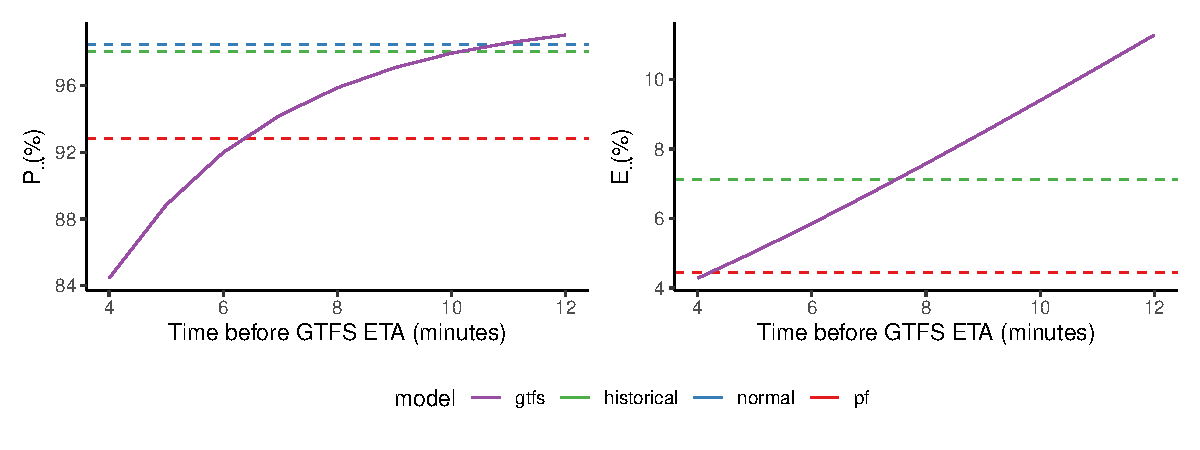
\includegraphics[width=\textwidth]{figure/model_results_pr_gtfs-1} 

}

\caption[Capture probability and expected wait times for schedule-delay predictions]{Capture probability and expected wait times for a traveller arriving $x$ minutes before the schedule-delay prediction. The relevant values for the three other methods are displayed by dashed lines.}\label{fig:model_results_pr_gtfs}
\end{figure}


\end{knitrout}



First, let us consider the probability of the bus arriving after the estimated arrival time, $\mathbb{P}_\ell$. Based on the data collected, a passenger would need to arrive at least 10~minutes before the \gls{eta} predicted by \Fsched{} to have a 97.5\% probability of catching the bus. To obtain the same probability as \Fpf{}, this would be a little more than 6~minutes before arrival. Now for the expected waiting time: to achieve the targetted 97.5\% chance of catching the bus, the passenger would arrive 10 minutes before the stated \gls{eta} which, from the figure on the right, has an expected waiting time of about 9~minutes. Arriving 6~minutes before yields an expected wait time of about 6~minutes, which is longer than the expected wait time under \Fpf{} (a little over 4~minutes), despite having the same probability of catching the bus.


We can also consider the reverse: a passenger would need to arrive no more than 4~minutes before the stated arrival time to have the same expected wait as \Fpf{}, giving them an 85\% chance of catching the bus compared to 93\% for \Fpf{}. For the remainder of this section, we use 6~minutes before the specified \gls{eta} to obtain a lower bound for \Fsched{}, and once more compare the probabilities as a function of time until arrival, stop sequence, and time of day.



\subsubsection{Time until arrival}

\Cref{fig:model_results_pr_time} shows $\mathbb{P}_m$, $\mathbb{P}_\ell$, and $\mathbb{E}_\ell$ computed at one-minute intervals for each of the four methods. \Fsched{} used a lower bound of $\hat\Tarr - 300$ (6~minutes before the point estimate). For the expected wait time, 5\% and 90\% quantiles are displayed as shaded regions. The dotted line in the expected waiting time graph represents the maximum possible waiting time; that is, the waiting time for a passenger already at the stop, given the bus is 10~minutes away, is 10~minutes.


\begin{knitrout}\small
\definecolor{shadecolor}{rgb}{0.969, 0.969, 0.969}\color{fgcolor}\begin{figure}
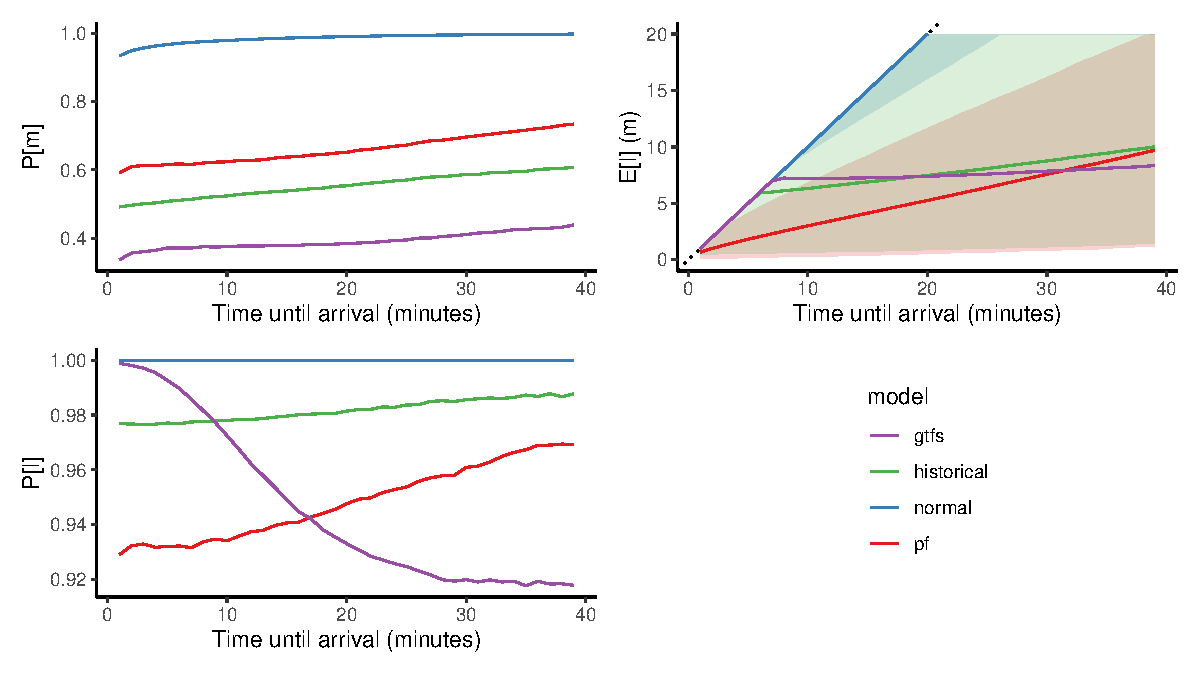
\includegraphics[width=\textwidth]{figure/model_results_pr_time-1} \caption[Capture probabilities and expected wait times for the models by time until the bus's actual arrival]{Capture probabilities and expected wait times for the models by time until the bus's actual arrival. Expected wait time (right) includes a shaded region for the 5 and 90\% quantiles of wait times.}\label{fig:model_results_pr_time}
\end{figure}


\end{knitrout}


The probability that the bus arrives after the point estimate (mean or median), $\mathbb{P}_m$, is more or less constant with a slight decrease as the bus nears the stop. \Fpf{} and \Fnorm{} are above the expected value of 50\%, though the latter is significantly higher. \Fnorm{} performs reasonably well, though it tends to underestimate arrival time the farther out the bus is, while \Fsched{} overestimates arrival time such that there is less than a 40\% chance of catching the bus if it is less than 20~minutes away.


For $\mathbb{P}_\ell$, we observe a different trend: \Fpf{} and \Fhist{} increase the further out the vehicle is; on the other hand with \Fsched{}, the probability decreases, an artefact of using a fixed lower bound. Once the bus is about 15~minutes away, the lower bound of \mbox{$\hat\Tarr - 300$} (\Fsched{} minus 6~minutes) is increasingly likely to result in a caught bus, while under \Fpf{} this probability is lower since the width of the interval decreases as fewer sources of variability remain.


Finally, we examine the expected waiting time, given a passenger arrives at the lower bound \emph{and} the bus arrives after it. \Fpf{} has a consistently shorter waiting time, though by about 30~minutes until arrival the three methods (excluding \Fnorm{}) are approximately the same. We see that the expected waiting time for \Fsched{} is more or less independent of time until arrival, which is to be expected since the width is fixed. The shaded reasons represent 5\% and 90\% quantiles of waiting time, revealing that \Fpf{} results in shorter waits, on average, when the bus is less than 10~minutes away. The Normal approximation tends towards overestimation of arrival time uncertainty, so expected waiting time is considerable if arriving at the lower estimate, indicating that \Fnorm{} is not a reliable choice for arrival time prediction.


\subsubsection{Stop sequence}

The same values were computed by stop sequence and displayed in \cref{fig:model_results_pr_stop}. \Fhist{} achieves the target probability of 50\%, while \Fpf{} is slightly above at about 60\%. Most notable is the steady decline in the reliability of \Fsched{}, dropping to about a one in three chance of catching the bus after stop 40 (assuming you arrive at the predicted \gls{eta}).


\begin{knitrout}\small
\definecolor{shadecolor}{rgb}{0.969, 0.969, 0.969}\color{fgcolor}\begin{figure}
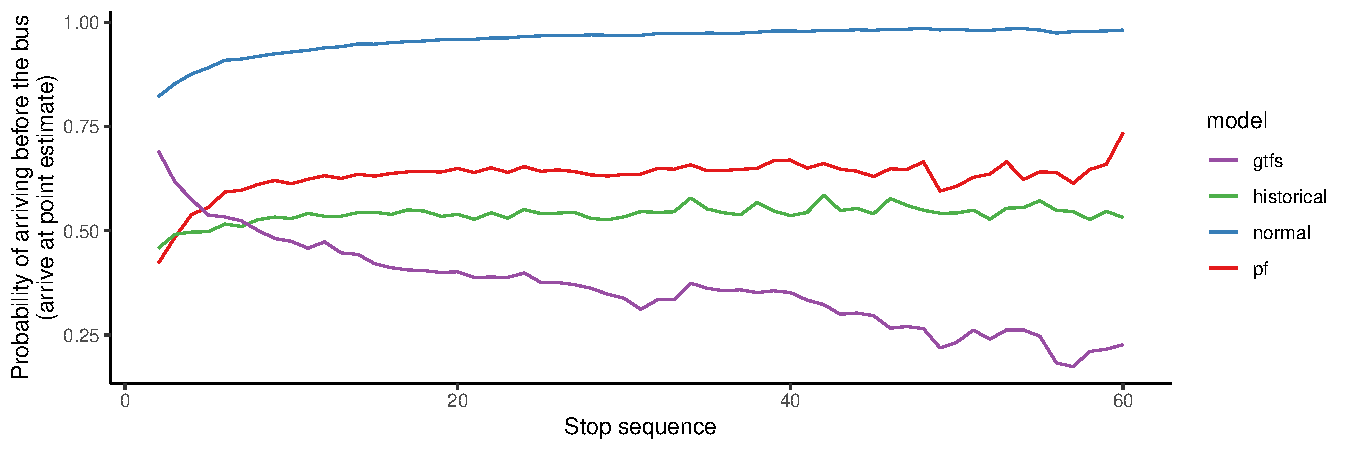
\includegraphics[width=\textwidth]{figure/model_results_pr_stop-1} \caption[Capture probabilities and expected wait times for the models by stop sequence]{Capture probabilities and expected wait times for the models by stop sequence. Expected wait time (right) includes a shaded region for the 5 and 90\% quantiles of wait times.}\label{fig:model_results_pr_stop}
\end{figure}


\end{knitrout}

Moving on to the lower 2.5\% quantile, $\mathbb{P}_\ell$, we expect 97.5\% probability of capture. We see that, as before, \Fpf{} overestimates arrival time slightly, with $\mathbb{P}_\ell$ of about 90\%, while for \Fsched{} it decreases with stop sequence. The associated wait time, $\mathbb{E}_\ell$, increases for all methods with increasing stop sequence \emph{except} for \Fsched{}, which decreases (remembering that the width is fixed). \Fpf{} has the lowest expected wait time, and the upper 90\% interval is lower than the mean for \Fsched{} for the first 20~stops. However, many stops with low indices are serviced within the first 5--10~minutes of the trip, thus inflating $\mathbb{P}_\ell$ under \Fsched{}.


\subsubsection{Time of day}

The probabilities and expected waiting time were calculated for 15~minute intervals for each of the models, as shown in \cref{fig:model_results_pr_timeofday}. The peak hour effects are one more visible and associated with an increased probability of arriving before the bus under \Fpf{} for both the median and 2.5\% quantile. For \Fsched{}, the probability of arriving before the bus decreases slightly during peak time. In the evening, we see the performance of \Fpf{} drop rapidly, likely due to the much-reduced probability of stopping (many evening services have low occupancy). Future work implementing more specific dwell time models could help to improve this.


\begin{knitrout}\small
\definecolor{shadecolor}{rgb}{0.969, 0.969, 0.969}\color{fgcolor}\begin{figure}
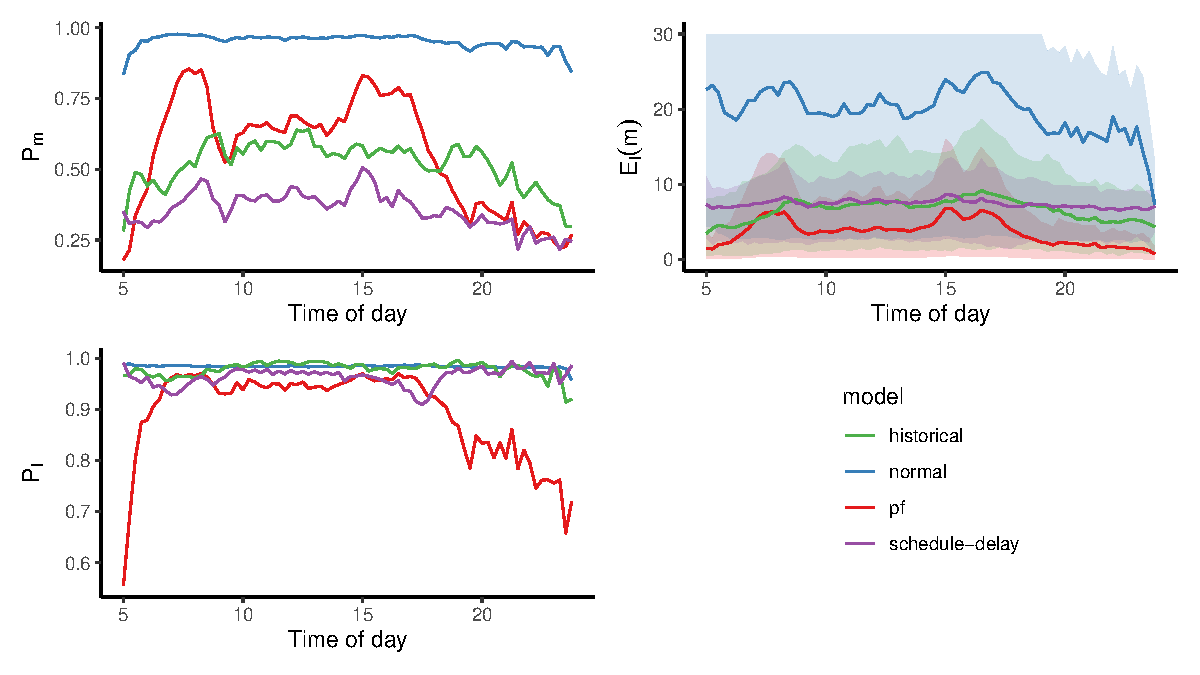
\includegraphics[width=\textwidth]{figure/model_results_pr_timeofday-1} \caption[Capture probabilities and expected wait times for the models by time of day]{Capture probabilities and expected wait times for the models by time of day. Expected wait time (right) includes a shaded region for the 5 and 90\% quantiles of wait times.}\label{fig:model_results_pr_timeofday}
\end{figure}


\end{knitrout}


We see much the same pattern with the expected wait time $\mathbb{E}_\ell$, which increase by a few minutes under \Fpf{} during peak times. There is little noticeable change for \Fsched{} and \Fhist{}. Even so, \Fpf{} consistently provides shorter expected wait times than \Fsched{}.


\subsection{Result summary}
\label{sec:prediction_model_comp_summary}

The results in \cref{sec:prediction_model_comp_stats,sec:prediction_model_comp_probs} demonstrate the relative accuracy and reliability of four methods of predicting the arrival time distribution at a stop. The particle filter (\Fpf{}) uses a sample of weighted particles representing the vehicle's state, along with the \rt{} traffic state, to approximate the distribution. On average, it is slightly more accurate than the currently used method (\Fsched{}), particularly when the bus is within 20~minutes of arriving and during the daytime off-peak period, and captures most of the uncertainty during this period (as per \gls{picp}).

As for the reliability of the estimates---that is, their use as an \gls{eta} for commuters---the \pf{} tends to underestimate arrival time, whereas the current method tends to \emph{overestimate} it. In terms of the application, the former is preferred, often resulting in a 30\% higher probability of catching the bus. The \pf{} provides an estimate of the arrival time distribution, allowing easy estimation of quantiles. We have seen that the lower bound is typically an overestimate, indicating that perhaps not enough variability is being included, or perhaps that more particles are needed. The presented results used $\tilde N = 200$, but future work could involve modifying this depending on the number of stops remaining along a route. However, the lower bound still gives a 90--95\% chance of catching the bus in most cases and has a significantly shorter wait time compared to the current method (assuming one arrives 6~minutes before the specified time). This difference indicates that the \pf{}, as well as providing improved prediction accuracy, can offer more reliability for passengers.


We saw that there were a few scenarios that could be attributed to much of the \pf{}'s weaker performance, namely peak times and evenings. Further work could be performed, particularly on forecasting network travel times, to improve these predictions. We also presented two other models. The Normal approximation (\Fnorm{}) demonstrated inferior performance in that it tended to overestimate arrival time uncertainty, a likely result of combining the mixtures. Historical data (\Fhist{}), in which the arrival time prediction distribution was based purely on the distribution of arrival time delays at stops along a route, performed admirably. It estimated the distribution quantiles well, but its reliability (at least compared to the other methods) decreased once the trip was underway and \rt{} information was available. It does, however, suggest that historical data should be used for prior predictions of arrival time: before a trip has registered with the \rt{} service, the best prediction of arrival time is \Fhist{}.
